\section{CAFE問題}\label{sec:background}

車両装備仕様問題は,\textbf{装備タイプ}とそれに付随する\textbf{装備オプション}から構成される.
装備タイプはエンジンやトランスミッションなどの装備の種類を表し,
装備オプションは,4気筒エンジン,6速ATなどの具体的な装備を表す.
以降,装備タイプをタイプ,装備オプションをオプションと呼ぶことにする.


\textbf{装備仕様}とは,タイプとオプションの組合せであり,
(エンジン, 4気筒), (トランスミッション, 6速AT)などの対の集合で表される.
車両装備仕様問題とは,与えられたタイプとオプションの集合から,
装備および燃費に関する制約を満たしつつ,販売台数を最大化する装備仕様を求める問題である.
本発表では,燃費に関する制約として,
企業別平均燃費 (Corporate Average Fuel Efficiency; CAFE)基準を採用する.
このCAFE基準は,自動車の燃費規制で,車種別ではなくメーカー全体で出荷台数を加味した
平均燃費を算出する方式である.日本では2020年度の燃費基準に採用されている.
以降では,CAFE基準による燃費制約を持つ車両装備仕様問題を\textbf{CAFE問題}と呼ぶ.

\begin{figure}[tb]
 \centerline {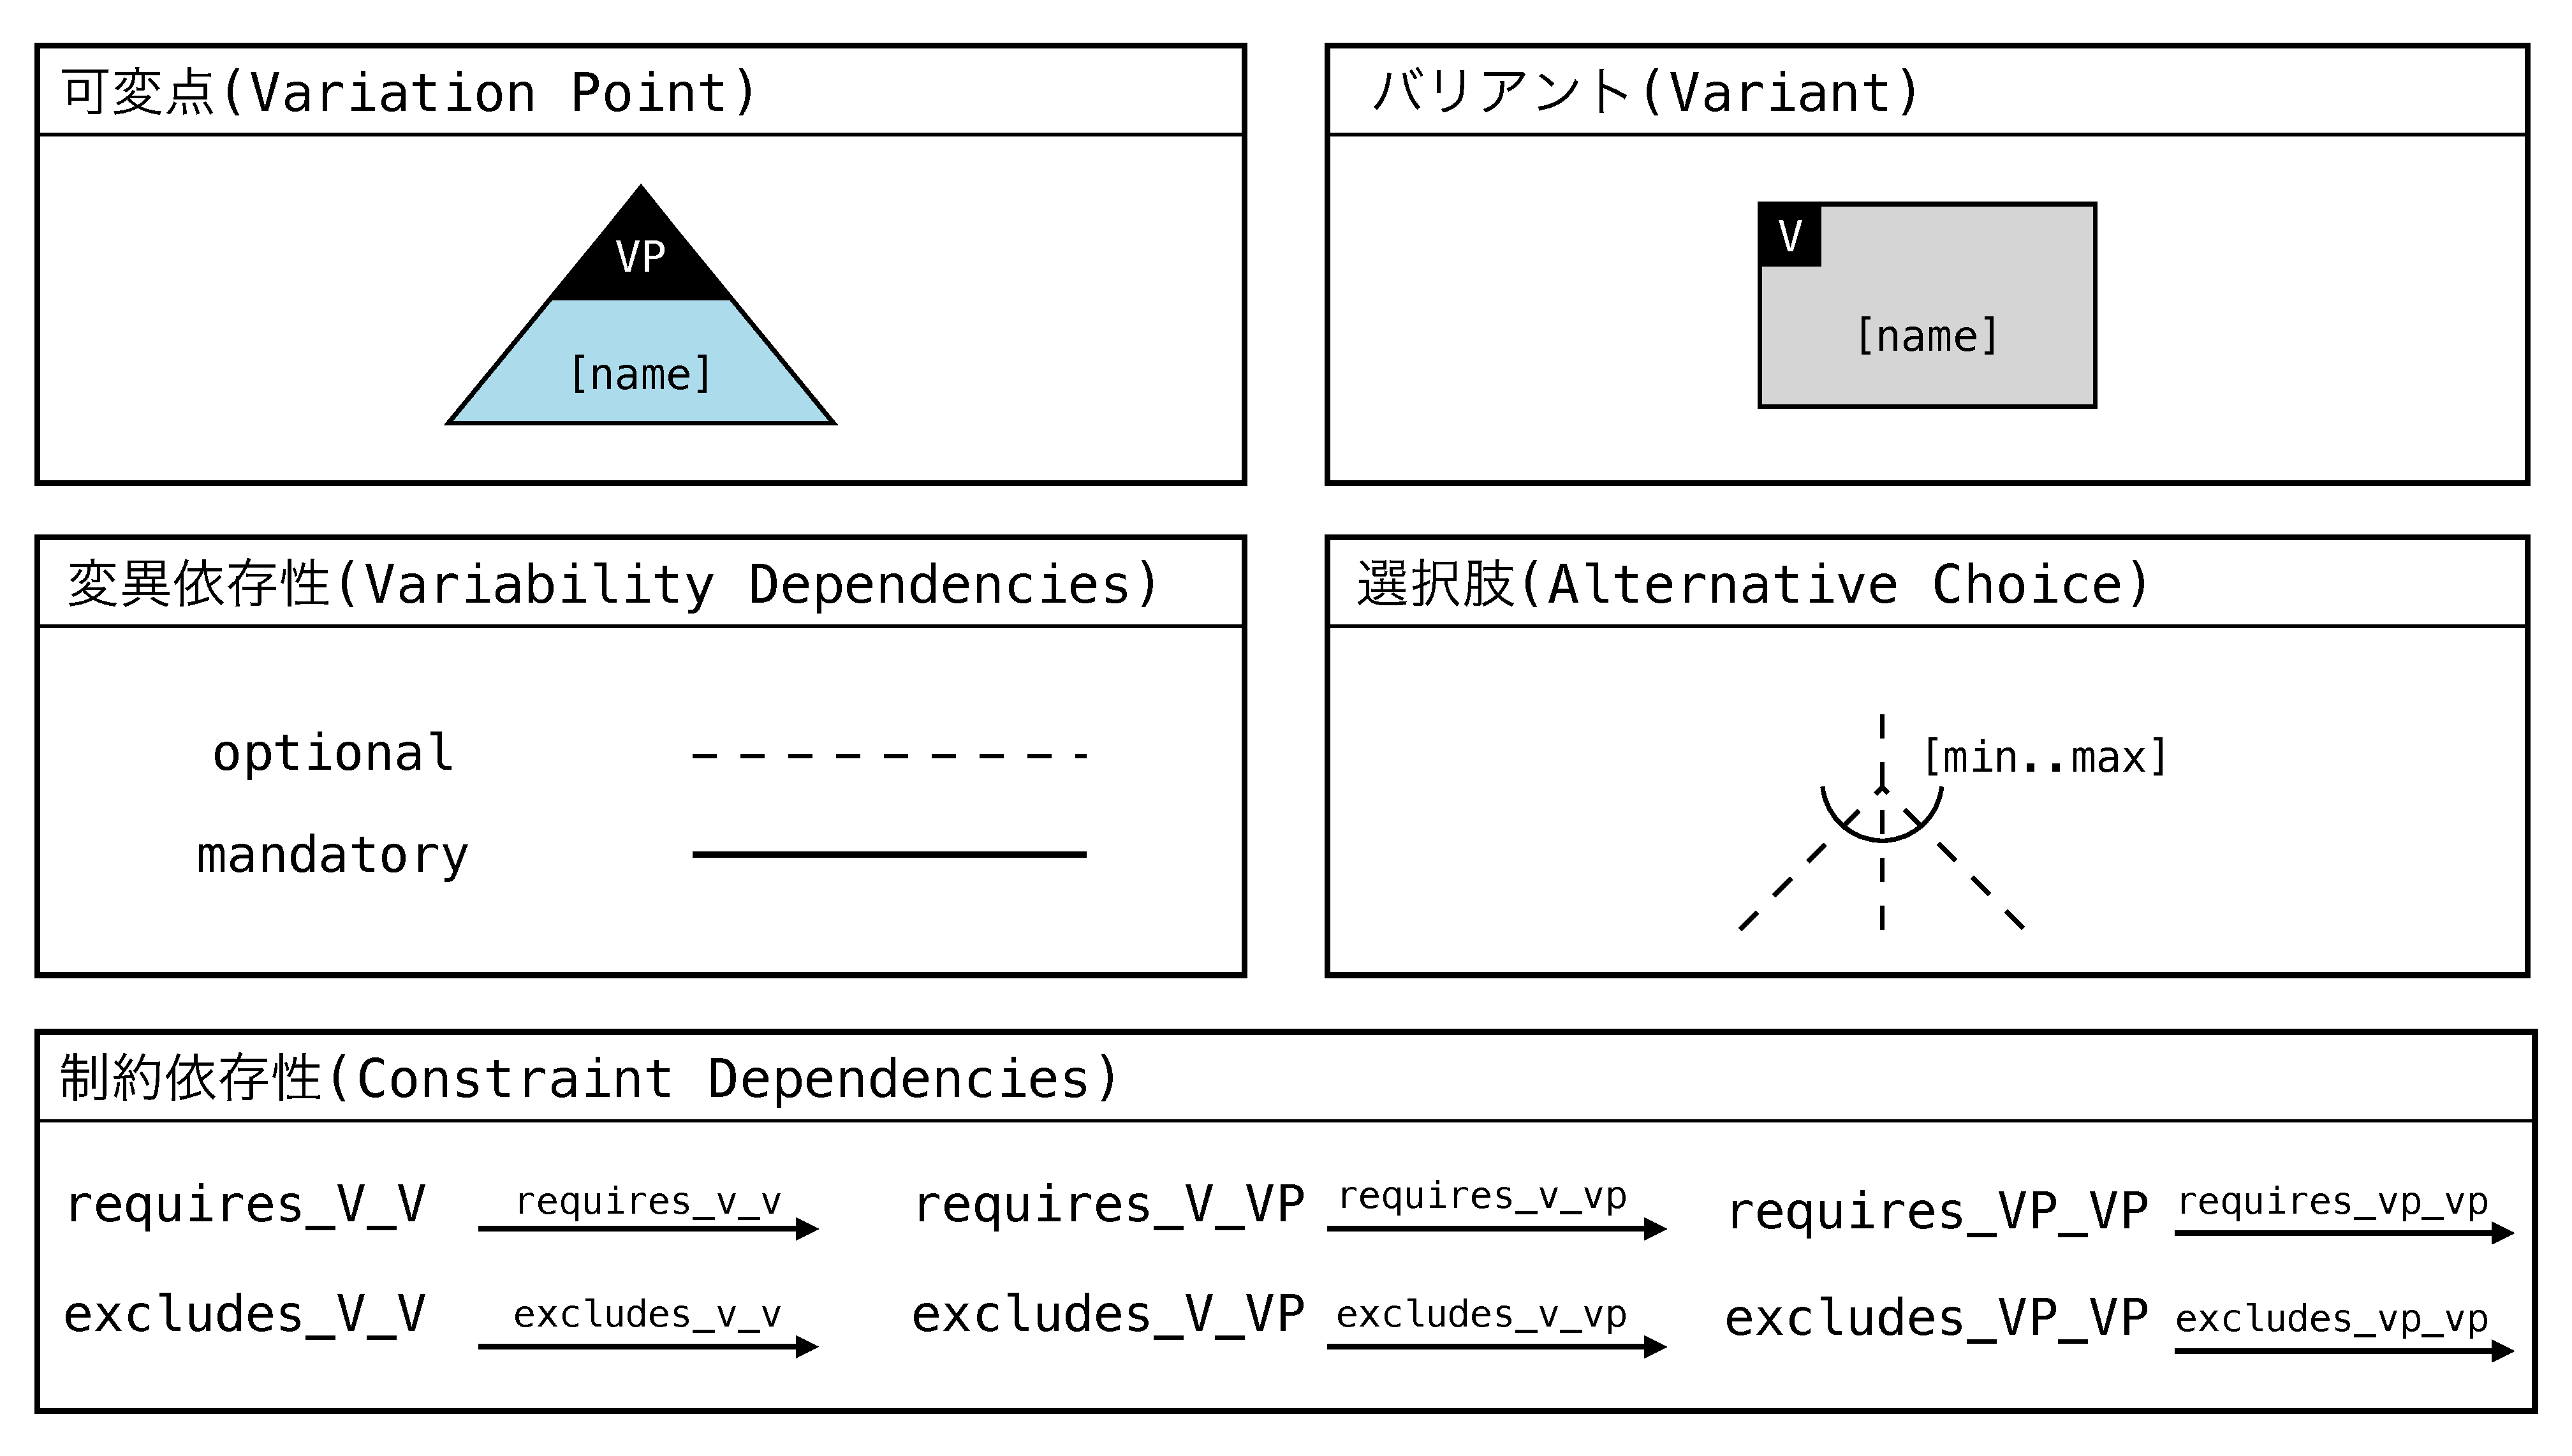
\includegraphics[width=\linewidth]{images/notation.eps}}
 \caption{OVM表記法\cite{Pohl05:sple}}
 \label{fig:ovm_notation}
\end{figure}

\begin{figure}[tb]
 \centerline {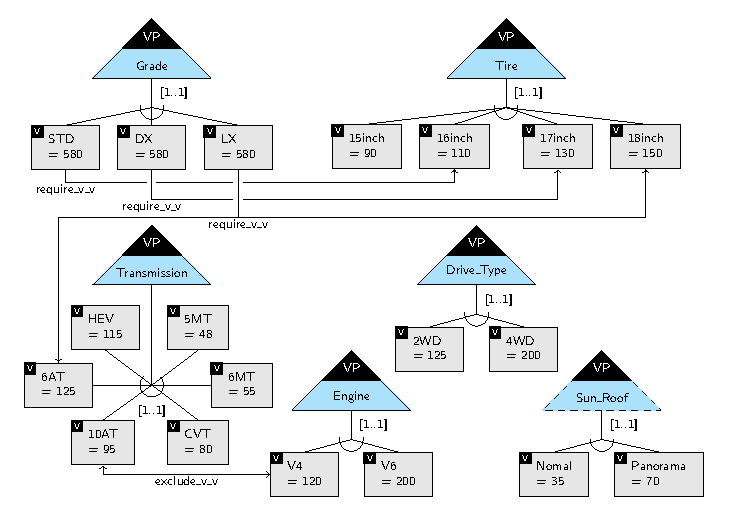
\includegraphics[width=\linewidth]{images/ovm01.eps}}
 \caption{CAFE問題の例}
 \label{fig:ovm_example}
\end{figure}

CAFE問題を表現する方法として,\textbf{可変性モデル(Orthogonal Variability Model;OVM)}
\cite{Pohl05:sple}を用いる.図\ref{fig:ovm_notation}
にOVMの表記法を示す.OVMでは,仕様ごとに変わりうる項目を
\textbf{可変点(Variation Point;VP)},その具体的なインスタンスを
\textbf{バリアント(Variant;V)}と呼ぶ.VPとVの対応関係には選択式(optional),
必須式(mondatory)があり,1つのVPに対して複数の選択式Vが存在する場合,
多重度によって制限された数のVが選択される.
また,VP間,V間,VとVP間に要求(require)や排除(exclude)の関係を定義することができる.



OVMで表現されたCAFE問題の例を図\ref{fig:ovm_example}に示す.CAFE問題においては,
タイプがVP,オプションがVとして表現され,Vの多重度はすべて[1:1]で,
各タイプごとにちょうど1つのオプションが選択される.
ただし,CAFE問題では図\ref{fig:ovm_example}のSun\_Roofのような必須ではないタイプが存在し,
このような選択式のタイプを表すVPは点線で囲まれている.
オプションには\textbf{IWR(Inertial Working Rating)}と呼ばれる重みのようなものが
それぞれ定められており,装備仕様ごとに選択されるオプションのIWRの和を引数として,
あらかじめ与えられているテーブルにより燃費と予想販売台数を得ることができる.
CAFE問題の燃費制約とは,装備仕様ごとの予想販売台数も加味した全体の平均燃費が与えられた
\textbf{CAFE基準値}以上にならなければならないという制約である.
3種類の装備仕様による燃費制約を式で表現すると,次のようになる.
\vspace{1em}
 \begin{displaymath}
  %\label{eq:cafe1} 
   \underbrace{
   \frac{Fe_{1} \times V_1 + Fe_{2} \times V_2 + Fe_{3} \times V_3 }{V_1 + V_2 + V_3}
   }_{\mbox{平均燃費}}
   \geq 
   \underbrace{t}_{\mbox{CAFE基準値}}
  \end{displaymath}
\vspace{1em}\\
ここでは,装備仕様$i$の燃費を$Fe_i$,予想販売台数を$V_i$としている.

\begin{table}[tb]
 \caption{CAFE問題の解の例}
 \begin{tabular}{l|c|c|c} \bhline
    \multicolumn{1}{c|}{装備}   & \multicolumn{3}{c}{装備仕様} \\ \cline{2-4}
                 & 1	& 2 	 & 3	\\  \hline
    Grade	 & STD	& DX	 & LX	\\
    Drive\_Type  & 2WD  & 2WD    & 2WD  \\
    Engine	 & V4	& V6	 & V6	\\
    Tire	 & 16	& 17	 & 18	\\
    Transmission & 5MT	& 6MT    & 10AT	\\
    Sun\_Roof    & -    & normal & -    \\ \hline
    IWR          & 983  & 1125   & 1180 \\ %\hline
    燃費(km/L)    & 10.2  & 8.9     & 8.5 \\ %\hline
    予想販売台数  & 745  & 1988   & 1171  \\ \hline
    平均燃費(km/L) & \multicolumn{3}{c}{\bf{9.0}} \\ 
    合計販売台数  & \multicolumn{3}{c}{\bf{3904}} \\ \hline
 \end{tabular}
 \label{tab:ovm_ans}
\end{table}

表\ref{tab:ovm_ans}にて,図\ref{fig:ovm_example}のCAFE問題の例に対する一つの解を示す.
このとき,求める装備仕様を3種類,CAFE基準値を9.0km/Lとし,それぞれの装備仕様のタイプGradeが
STD,DX,LXであるものとする.
各装備仕様の列に,それぞれのタイプで選択されるオプションが示されており,IWRの和から
燃費と予想販売台数が算出され,これらの値から全体の平均燃費と合計の販売台数が求められる.






% - CAFE問題の定義
% - OVMの解説
% - CAFE問題をOVMで表現
%   - 必須VPの説明どうする?既存のOVMにはない考え方
% - CAFE問題の各種制約をOVMになぞらえて解説
% - 解の例